\documentclass[xcolor=table, 10pt, aspectratio=1610]{beamer}

%\usepackage{arev}
\usepackage{amsmath,amssymb,amscd}
\usepackage{dsfont}
\usepackage{mathrsfs}
\usepackage{yfonts}
\usepackage{bm}
\usepackage{graphicx}
\usepackage{tabularx}
\usepackage{animate}
\usepackage{pifont}
\usepackage{ulem}
%\usepackage{mathtools}
%\usepackage{ifthen}

%\usepackage{xeCJK}
%\usepackage{fontspec}
%\newfontfamily\cjkfont{PingFang SC}
%\setCJKmainfont{PingFang SC}
\newcolumntype{x}{>{\centering\arraybackslash}X}
\renewcommand{\arraystretch}{1.5}
\newcommand{\uone}{\mathrm U(1)}
\DeclareMathOperator{\img}{img}

\usepackage{tikz}
	\usetikzlibrary{calc}
	\usetikzlibrary{arrows,shapes, positioning, matrix}
	\usetikzlibrary{decorations.markings}
	\tikzset{>=stealth}
	\tikzstyle arrowstyle=[scale=1]
	\tikzstyle directed=[postaction={decorate,decoration={markings,
 	   mark=at position .15 with {\arrow[arrowstyle]{stealth}}}}]
\tikzstyle string=[thick,postaction={decorate,decoration={markings,
    mark=at position .55 with {\arrow[arrowstyle]{stealth}}}}]
\tikzstyle dual_string=[dashed,postaction={decorate,decoration={markings,
    mark=at position .55 with {\arrow[arrowstyle]{stealth}}}}]

\tikzstyle dw=[thick,postaction={decorate,decoration={markings,
    mark=at position 1 with {\arrow[arrowstyle]{stealth}}}}]
\tikzstyle group=[mbg]
\newcommand*{\halfway}{0.5*\pgfdecoratedpathlength+.5*8pt}\tikzstyle arrowstyle=[scale=1]
\newcommand*{\halfwayb}{0.5*\pgfdecoratedpathlength}
\tikzstyle arrowstyle=[scale=1]
\tikzstyle fermion=[thick,postaction={decorate},decoration={markings,
    mark=at position \halfway with {\arrow[arrowstyle]{latex}}}]
\tikzstyle fermion2=[thick,postaction={decorate},decoration={markings,
        mark=at position \halfwayb with {\arrow[arrowstyle]{latex}}}]

\usepackage{pgffor}
\newcommand{\mb}[1]{\mathbf{#1}}
\renewcommand{\cal}[1]{\mathcal{#1}}

\newcommand{\ag}[2]{#1_\mb{#2}}
\newcommand{\cohosub}[1]{\scalebox{0.72}{\textswab{#1}}}
\newcommand{\cohosubsub}[1]{\scalebox{0.6}{\textswab{#1}}}
\newcommand{\coho}[1]{\textswab{#1}}

\DeclareMathOperator{\tr}{Tr}
\DeclareMathOperator{\im}{Im}
\DeclareMathOperator{\re}{Re}

\mode<presentation>
{
  %\usetheme{Warsaw}
  % or ...
  %\useoutertheme{rectangle}
  \setbeamertemplate{frametitle}[default][center]
  \defbeamertemplate{itemize item}{flat}{\begin{pgfpicture}{-1ex}{0ex}{1ex}{2ex}
      \pgfpathcircle{\pgfpoint{0pt}{.6ex}}{0.6ex}
      \pgfusepath{fill}
    \end{pgfpicture}%
  }
  \defbeamertemplate{itemize subitem}{flat}{\footnotesize\raise0.5pt\hbox{\textbullet}}
  \defbeamertemplate{itemize subsubitem}{flat}{\footnotesize\raise0.5pt\hbox{\textbullet}}

  %\useinnertheme{circles}
  \setbeamertemplate{items}[flat]
  \setbeamertemplate{sections/subsections in toc}[circle]
  \setbeamertemplate{blocks}[rounded]
  \setbeamertemplate{title page}[default][colsep=-4bp,rounded=true]
  \setbeamertemplate{part page}[default][colsep=-4bp,rounded=true]
  \setbeamercovered{transparent}
  %\usecolortheme{spruce}
  %\definecolor{THU}{RGB}{116,61,130}
  \definecolor{mbg}{RGB}{0,0,160}
  \setbeamercolor*{palette primary}{fg=white,bg=mbg}
  \setbeamercolor*{titlelike}{parent=palette primary}
  \setbeamercolor*{structure}{fg=mbg}
  \setbeamercolor{frametitle}{fg=white,bg=mbg}
  % or whatever (possibly just delete it)
  \setbeamercolor{block title}{bg=mbg,fg=white}
  \setbeamercolor{block body}{bg=mbg!15}


  \addtobeamertemplate{navigation symbols}{}{ \hspace{1em}%
    \usebeamerfont{footline}%
    \insertframenumber / \inserttotalframenumber }
}


%\usepackage[english]{babel}
% or whatever

%\usepackage[latin1]{inputenc}
% or whatever

%\usepackage{times}
%\usepackage[T1]{fontenc}
% Or whatever. Note that the encoding and the font should match. If T1
% does not look nice, try deleting the line with the fontenc.

\title[Space-group SPTs] % (optional, use only with long paper titles)
{Real-Space Classification of Bosonic Space-Group SPTs}

\author[Y Qi] % (optional, use only with lots of authors)
{Yang~Qi}
% - Give the names in the same order as the appear in the paper.
% - Use the \inst{?} command only if the authors have different
%   affiliation.

\institute[Fudan] % (optional, but mostly needed)
{Department of Physics, Fudan University}
% - Use the \inst command only if there are several affiliations.
% - Keep it simple, no one is interested in your street address.

%\date{2016 Annual Meeting of Fudan CFTPP} % (optional, should be abbreviation of conference name)
%{Fudan University, Oct 13 2015}
\date{MIT, Aug. 20 2018}
% - Either use conference name or its abbreviation.
% - Not really informative to the audience, more for people (including
%   yourself) who are reading the slides online

\subject{Theoretical Physics}
% This is only inserted into the PDF information catalog. Can be left
% out.



% If you have a file called "university-logo-filename.xxx", where xxx
% is a graphic format that can be processed by latex or pdflatex,
% resp., then you can add a logo as follows:

\pgfdeclareimage[height=1cm]{university-logo}{../resources/fudan}
\logo{\pgfuseimage{university-logo}}

\AtBeginSection[]
{
  \begin{frame}<beamer>{Outline}
			\tableofcontents[currentsection,currentsubsection]
			\begin{center}
				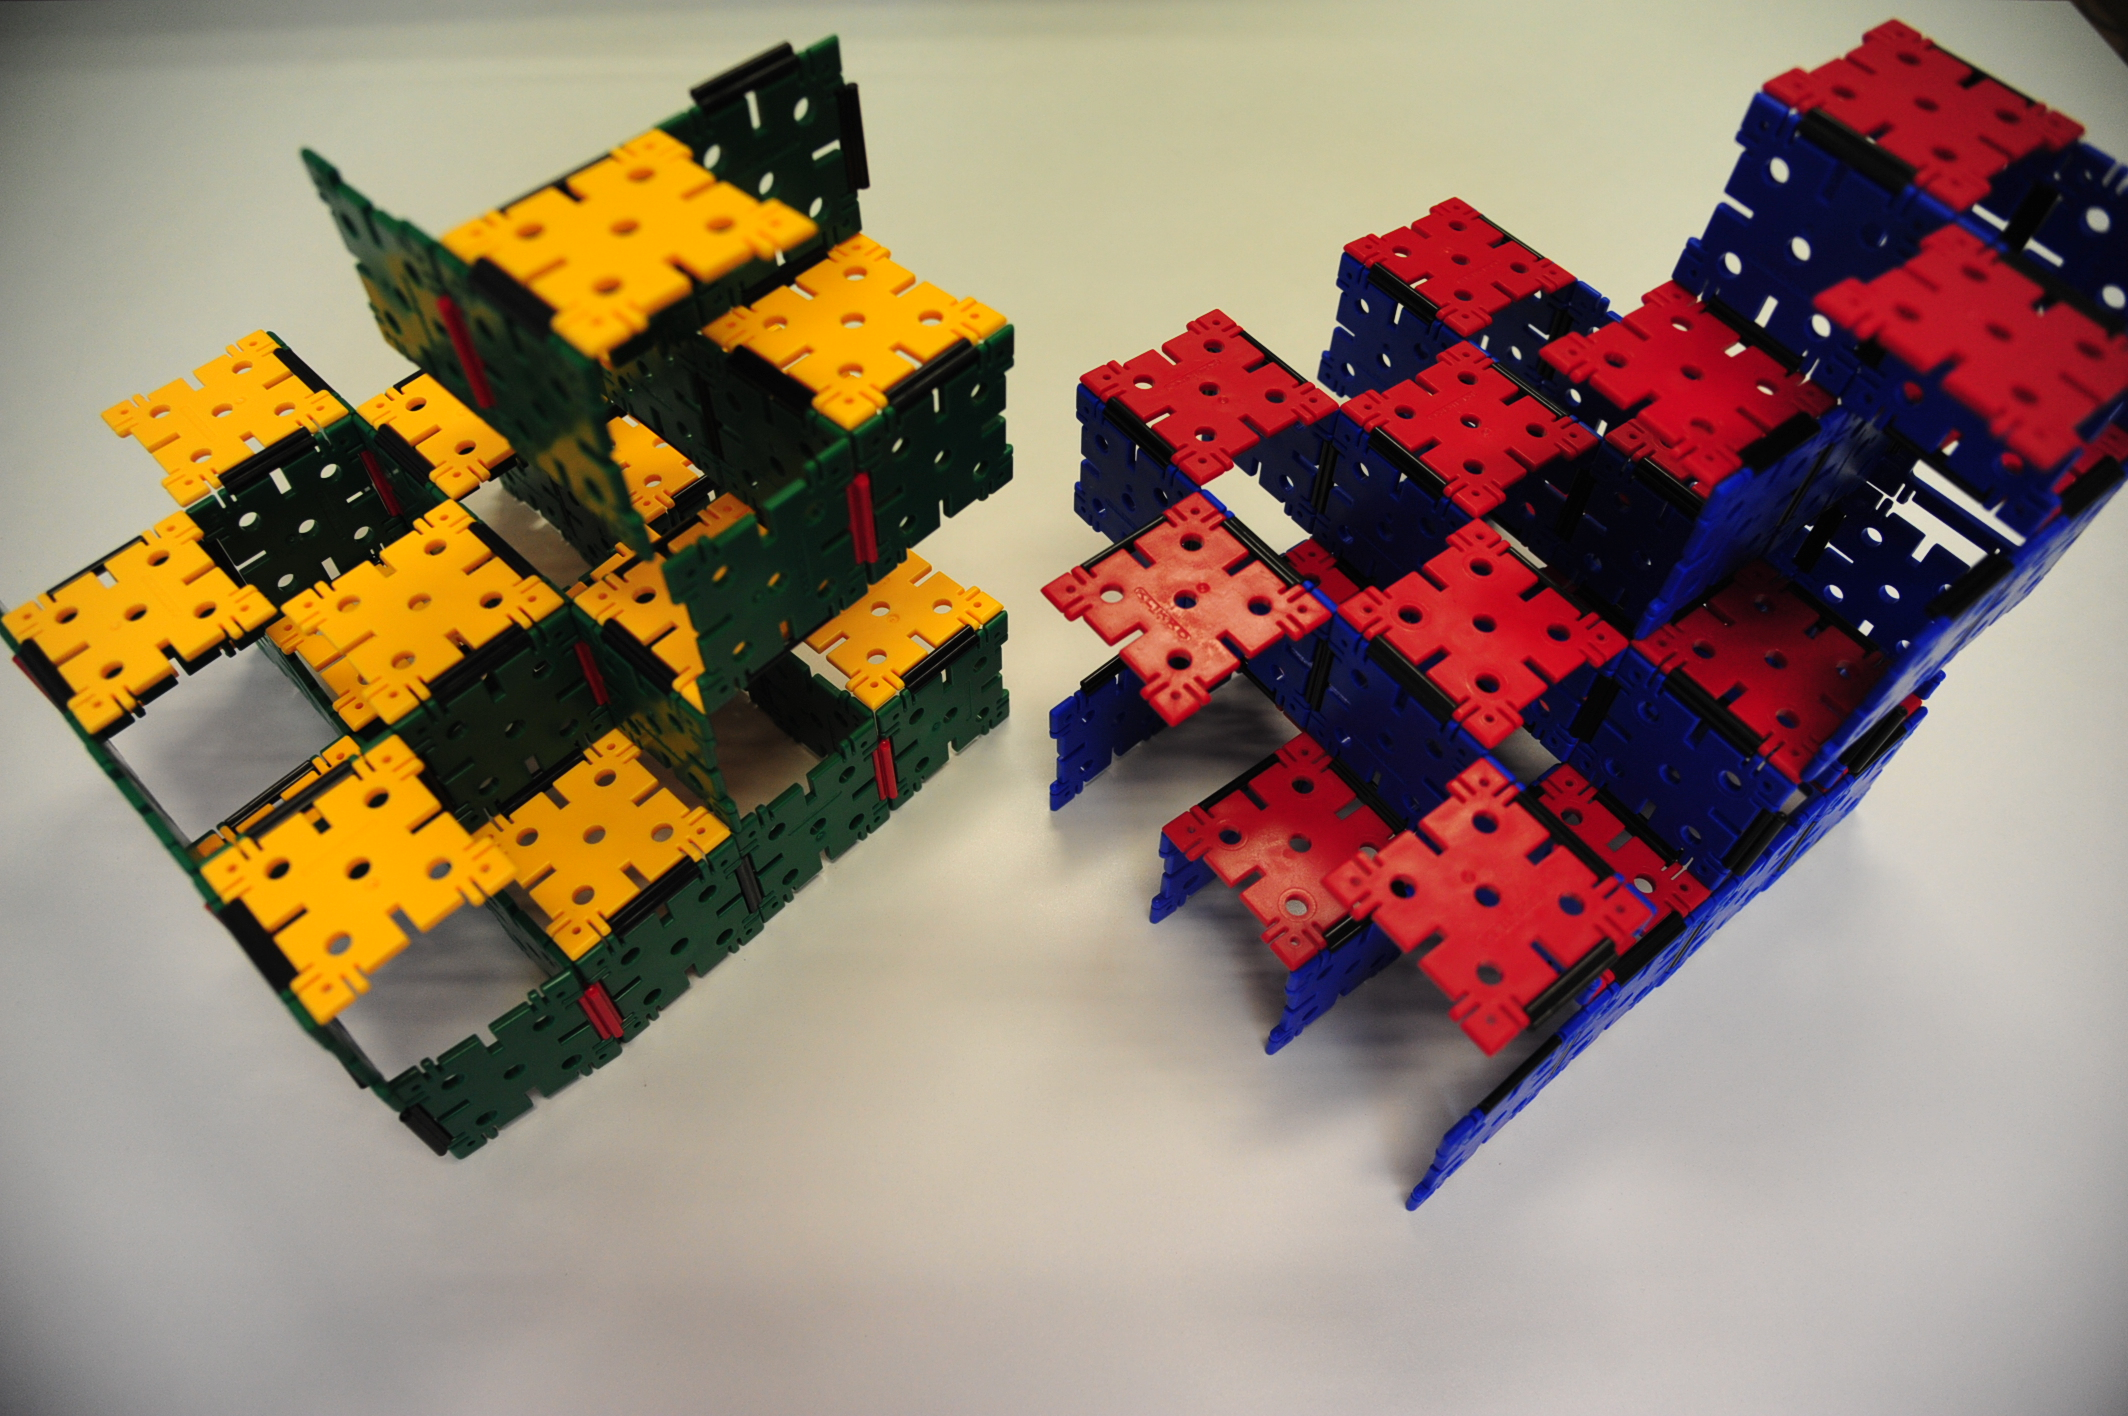
\includegraphics[height=4cm]{toys}
			\end{center}
  \end{frame}
}


% Delete this, if you do not want the table of contents to pop up at
% the beginning of each subsection:

\begin{document}

\begin{frame}
  \frametitle{SPT classification: progress and remaining challenges}
  \begin{enumerate}
  \item[\ding{51}] Bosonic SPT: group cohomology.
  \item[\ding{51}] Free-fermion SPT: K-theory.
  \item[?] Interacting-fermion SPT: generalized cohomology. Almost done but a few challenges remain.
  \item[\ding{51}] Crystalline SPT: use Crystalline equivalence principle. Thorngren \& Else, PRX 2018.
  \item[\ding{51}] Computation: GAP package at \url{https://github.com/yangqi137/SptSet}.
  \end{enumerate}
\end{frame}

\begin{frame}
  \frametitle{Crystalline SPT: real-space construction}
  %\begin{columns}
    %\column{.6\textwidth}
    \begin{itemize}
    \item Assemble a crystalline SPT in real space using a spectral sequence. Zhida Song, Chen Fang \& YQ; Else \& Thorngren.
    \item Can reproduce all bosonic SPT states.
    \item Compute high-order boundary anomalies for HOSPTs: Chen Fang and YQ, to appear.
    \item Next: free-fermion HOSPTs?
    \end{itemize}
    
    %\column{.4\textwidth}
    \begin{center}
      \begin{tikzpicture} [scale=1.5]
        \fill [blue!50] (0,0)--(1,0)--(1.5,.5)--(1.5,1.5)--(0.5,1.5)--(0,1)--(0,0);
        \draw [thick,white] (0,0)--(1,0)--(1,1)--(0,1)--(0,0);
        \draw [thick,white] (1,0)--(1.5,.5)--(1.5,1.5)--(1,1);
        \draw [thick,white] (1.5,1.5)--(0.5,1.5)--(0,1);
        \draw [thick,white] (0,0)--(.5,.5)--(.5,1.5);
        \draw [thick,white](.5,.5)--(1.5,.5);
        \fill [white] (0,0) circle (2pt);
        \fill [white] (1,0) circle (2pt);
        \fill [white] (0,1) circle (2pt);
        \fill [white] (1,1) circle (2pt);
        \fill [white] (0.5,0.5) circle (2pt);
        \fill [white] (1.5,0.5) circle (2pt);
        \fill [white] (0.5,1.5) circle (2pt);
        \fill [white] (1.5,1.5) circle (2pt);
      \end{tikzpicture}
      \begin{tikzpicture} [scale=1.5]
        \fill [blue!50] (0,0)--(1,0)--(1.5,.5)--(1.5,1.5)--(0.5,1.5)--(0,1)--(0,0);
        \draw [thick,black!50!green] (0,0)--(1,0)--(1,1)--(0,1)--(0,0);
        \draw [thick,thick,black!50!green] (1,0)--(1.5,.5)--(1.5,1.5)--(1,1);
        \draw [thick,thick,black!50!green] (1.5,1.5)--(0.5,1.5)--(0,1);
        \draw [thick,thick,black!50!green] (0,0)--(.5,.5)--(.5,1.5);
        \draw [thick,thick,black!50!green](.5,.5)--(1.5,.5);
        \fill [white] (0,0) circle (2pt);
        \fill [white] (1,0) circle (2pt);
        \fill [white] (0,1) circle (2pt);
        \fill [white] (1,1) circle (2pt);
        \fill [white] (0.5,0.5) circle (2pt);
        \fill [white] (1.5,0.5) circle (2pt);
        \fill [white] (0.5,1.5) circle (2pt);
        \fill [white] (1.5,1.5) circle (2pt);
      \end{tikzpicture}
      \begin{tikzpicture} [scale=1.5]
        \fill [blue!50] (0,0)--(1,0)--(1.5,.5)--(1.5,1.5)--(0.5,1.5)--(0,1)--(0,0);
        \draw [thick,black!50!green] (0,0)--(1,0)--(1,1)--(0,1)--(0,0);
        \draw [thick,thick,black!50!green] (1,0)--(1.5,.5)--(1.5,1.5)--(1,1);
        \draw [thick,thick,black!50!green] (1.5,1.5)--(0.5,1.5)--(0,1);
        \draw [thick,thick,black!50!green] (0,0)--(.5,.5)--(.5,1.5);
        \draw [thick,thick,black!50!green](.5,.5)--(1.5,.5);
        \fill [red] (0,0) circle (2pt);
        \fill [red] (1,0) circle (2pt);
        \fill [red] (0,1) circle (2pt);
        \fill [red] (1,1) circle (2pt);
        \fill [red] (0.5,0.5) circle (2pt);
        \fill [red] (1.5,0.5) circle (2pt);
        \fill [red] (0.5,1.5) circle (2pt);
        \fill [red] (1.5,1.5) circle (2pt);
      \end{tikzpicture}
    \end{center}
  %\end{columns}

  \end{frame}

\begin{frame}
  \frametitle{Question: topology and strongly-correlated systems}
  \begin{enumerate}
  \item \sout{Gapped} Gapless topological phases: properties of gapless quantum spin liquids, etc.
  \item CFT and other gapless phases vs gapped topological phases in one-higher dimensions: dual higher symmetry; disorder operator.
    Wenjie Ji, Xiao-Gang Wen, Cenke Xu, Meng Cheng, Zi Yang Meng, etc.
  \item 4-pt and higher-order correlation functions: experiments; beyond-MF correlations; bootstrap.
  \end{enumerate}
\end{frame}

\end{document}